\RequirePackage[2020-02-02]{latexrelease}
\documentclass{ntuthesis}


\usepackage{amsmath, amssymb, amsthm}
\usepackage{bm, bbm}
\usepackage{physics}
\usepackage{natbib}
% \usepackage{newtxmath}
\usepackage{appendix}
\usepackage[hang]{footmisc}
\usepackage{caption}    % for subfigure
\usepackage{subcaption} % for subfigure
\usepackage[compact]{titlesec}    % remove redundant spacing
\usepackage{times}
\usepackage{threeparttablex,longtable}
\usepackage{booktabs}
\usepackage{multirow}
\usepackage{afterpage}  % load the afterpage package
\usepackage[inline]{enumitem}   % can get rid of new line
\usepackage[section]{placeins}
\usepackage{lscape}   % landscape
\usepackage{verbatim}
\usepackage{color}
\usepackage{url}
\usepackage{graphicx}
\usepackage{setspace}
\usepackage{array}
\usepackage{wallpaper}
\usepackage[hidelinks]{hyperref}
\usepackage[printwatermark]{xwatermark}
\usepackage[capposition=top]{floatrow}
\usepackage{chngcntr}
\newcommand{\BL}{\emph{Bitcoin Law}}
\newcommand{\chivo}{\emph{Chivo Wallet}}
\newcommand{\BC}{\emph{Bitcoin City}}

\DeclareMathOperator*{\argmin}{arg\,min}

\newcommand{\refeq}[1]{Equation~({\ref{#1}})}

\counterwithout{equation}{chapter}
\counterwithout{figure}{chapter}
\counterwithout{table}{chapter}
% Using the tex-text mapping for ligatures etc.
\defaultfontfeatures{Mapping=tex-text}
% Set the default fonts
\setmainfont{Times New Roman}
\setCJKmainfont[AutoFakeBold=true,AutoFakeSlant=true]{標楷體}
%\setCJKmainfont[BoldFont={粗楷體},ItalicFont={斜楷體}]{標楷體}
\setlength\footnotemargin{10pt}

\theoremstyle{definition}
\newtheorem{definition}{Definition}
\newtheorem{proposition}{Proposition}

\ifdefined\firstpage

  \def\withwatermark{1}
  \ifdefined\withwatermark
    \newsavebox\mybox
    \savebox\mybox{\tikz[opacity=0.5]\node{\includegraphics{watermark.pdf}};}
    \newwatermark*[allpages,xpos=6.1725cm,ypos=10.5225cm,scale=0.5]{\usebox\mybox}
  \fi

  % digital object identifier
  \ifdefined\withdoi
    \insertdoi
  \fi
\fi

\makeatletter
\AtBeginDocument{
  \hypersetup{
    pdftitle={\@titleen},
    pdfauthor={\@authoren},
    pdfsubject={\@typeen{} \@classen},
    pdfkeywords={\@keywordsen}
  }
}
\makeatother

% Your information goes here
% author: Tz-Huan Huang [http://www.csie.ntu.edu.tw/~tzhuan]

% ----------------------------------------------------------------------------
% "THE CHOCOLATE-WARE LICENSE":
% Tz-Huan Huang wrote this file. As long as you retain this notice you
% can do whatever you want with this stuff. If we meet some day, and you think
% this stuff is worth it, you can buy me a chocolate in return Tz-Huan Huang
% ----------------------------------------------------------------------------

% Syntax: \var{English}{Chinese}
\university{National Taiwan University}{國立臺灣大學}
\college{College of Social Science}{社會科學院}
\institute{Department of Economics}{經濟學系}
\title{Examining the Chinese Debt-Trap Diplomacy}{檢視中國債務陷阱}
\author{Chia-Wei Chen}{陳家威}
\studentid{R10323045}
\advisor{Tai-kuang Ho, Ph.D.}{何泰寬 博士}
\defenseyear{2023}{112}
\defensemonth{June}{6}
\defenseday{28}
\doi{doi:10.6342/NTU2017XXXXX}
\keywords{Debt-Trap Diplomacy, Belt and Road Initiative, Sovereign Debt, Optimal Default}{債務陷阱外交、一帶一路、主權債務、最適違約決定}


\titleformat{\chapter}                      % 設置 Chapter 格式
{\Huge\bfseries}                            % 定義 format
{Chapter~\thechapter:~}              		        % 定義 label
{1em}                                       % 定義 sep
{} 
\begin{document}

\frontmatter

\makecover

\ifdefined\excludefirstpage

  \def\withwatermark{1}
  \ifdefined\withwatermark
    \newsavebox\mybox
    \savebox\mybox{\tikz[opacity=0.5]\node{\includegraphics{watermark.pdf}};}
    \newwatermark*[allpages,xpos=6.1725cm,ypos=10.5225cm,scale=0.5]{\usebox\mybox}
  \fi

  % digital object identifier
  \ifdefined\withdoi
    \insertdoi
  \fi
\fi

% \makecertification

% \begin{acknowledgementszh}

這個論文能夠順利的完成 ,我首先要感謝我的指導老師,何泰寬教授。

這其實是我的第三個題目。第一個題目是透過agent-based model 模擬CBDC,但考慮時間後及時停損。第二個題目是關於薩爾瓦多採用比特幣作為法定貨幣對直接投資的影響,但因為中間的影響管道實在缺乏一個令人信服的經濟管道,所以在何老師的建議下更換為現在這個題目。此時已經五月初,因此若不是何老師在接下來三個月細心的協助跟指導,我無法想像我能在短時間之內完成我的論文。
老師對於科學方法的嚴謹,是我完成這篇論文後最大的收穫。剛接收到這個題目的第三周,我就急著糊裡糊塗的進行模型校準,跑了文獻中的程式碼,最後出來的結果慘不仁賭。
在一次的meeting之後當頭棒喝,發現我的理解有很大的錯誤。於是我重新細讀各種文獻,重新理解做法,仔細認識我的研究對象的背景,經過了將近一個月的理解與嘗試後,才終於如願地跑出這個令人振奮的結果。因為何老師對學術研究高規格的要求,我對社會科學的實證研究態度有了重大的轉變,我由衷的感激,也十分慶幸能接受何老師的指導。

感謝口試委員朱玉琦老師、葉國俊老師、楊宗翰老師、以及楊茜文老師對於論文內容的修改建議。各位老師對於本研究的想法與建議,都使這份研究更加具有學術價值。另外,雖然 agent-based model 最後沒有用於我的論文,我還是感謝陳樹衡老師開放旁聽有關此一工具的課程。

在幾次更換題目的期間,我的心情其實是十分低落且緊張的。我很感謝姵璇在這段時間對我的鼓勵以及陪伴,在這段期間願意聆聽我的各種苦訴,在我覺得好像什麼都做不好的時候願意跟我研究如何將實習時很冗的工作自動化,給我很大的信心。我也要感謝宗弘、霖東、以及 651室的張翔、呂越,隨時跟我分享一些新奇的經濟學想法;感謝鑫君做為好鄰居協助統計、偉駿與我共同研究數據處理還有程式設計、宇杰協助Latex的設定、以及Oscar 協助我進行西班牙語文件的翻譯。口試前一周,也感謝馥暄以及芳語協助練習。感謝系辦禮禎協助所有遠距口室相關事宜。我也要感謝我的家人,無論是什麼時候都在支持著我的決定,放心的讓我挑戰我先前從未接觸過的經濟。

在我的研究生涯中還有太多可以感謝的人,無論事情是大事小,我都很感激你們的存在。

I would like to express my gratitude to Dr. Hinrichsen for sharing the code and engaging in discussions regarding the default set graph. Without your generosity, I would not have been able to complete my thesis. Additionally, I extend my thanks to Dr. Na and Dr. Schmitt-Grohé for their insightful discussions on the model, which helped clarify important concepts for me. Lastly, I am truly thankful for Mr. Sperr's prompt reply and assistance in proofreading my thesis just a week before my oral defense.
\\[2em]
\begin{flushright}
    陳家威 僅誌\\
    於國立臺灣大學經濟學研究所

    中華民國一一二年七月二十日
\end{flushright}

\end{acknowledgementszh}

% \begin{acknowledgementsen}
% I'm glad to thank\ldots 
% \end{acknowledgementsen}

% \begin{abstractzh}
關於中國在「一帶一路」倡議下向接受國家提供的過度貸款是否導致這些國家陷入高度債務並最終陷入「債務陷阱」的爭議仍然存在。本論文旨在通過運用一個主權債務模型的校準,從實證角度對這個議題進行考察。具體而言,本研究聚焦於兩個在中國戰略上具有重要地位的國家 --- 斯里蘭卡和巴基斯坦。

研究結果確認了這兩個國家在接受大量貸款後確實陷入了債務違約的狀態。基於這些結果,本研究提出了兩個債務陷阱的類別,並將斯里蘭卡和巴基斯坦分別歸入不同的類別。這種分類方法為債務陷阱外交的相關文獻提供了客觀的評估和呈現方式。
\bigbreak
\noindent \textbf{關鍵字:}{\, \makeatletter \@keywordszh \makeatother}
\end{abstractzh}

\begin{abstracten}

    Ongoing debates remain surrounding whether the excessive loans provided by China under the Belt and Road Initiative lead to high indebtedness and eventual ``debt traps'' for recipient countries. This thesis empirically examines this topic through the calibration of a sovereign debt model. Specifically, the study focuses on two strategically important countries --- Sri Lanka and Pakistan.
    The research findings validate the notion that these two countries indeed fell into the default set once they received substantial loan amounts, allowing for two categories of debt traps into which Sri Lanka and Pakistan reside. This categorization offers an objective assessment and presentation method within the literature on debt-trap diplomacy.
    \bigbreak
\noindent \textbf{Keywords:}{\, \makeatletter \@keywordsen \makeatother}
\end{abstracten}

\begin{comment}
\category{I2.10}{Computing Methodologies}{Artificial Intelligence --
Vision and Scene Understanding} \category{H5.3}{Information
Systems}{Information Interfaces and Presentation (HCI) -- Web-based
Interaction.}

\terms{Design, Human factors, Performance.}

\keywords{Region of interest, Visual attention model, Web-based
games, Benchmarks.}
\end{comment}


% \tableofcontents
% \listoffigures
% \listoftables

\mainmatter


\chapter{Introduction}
As China's economic influence continues to grow, its lending practices to developing countries have come under scrutiny.
The concept of ``debt-trap diplomacy'', whereby China extends excessive loans to countries and places a debt burden upon them in exchange for political or economic concessions, has become a topic of heated debate \citep{Chellaney_2017}.

From the political science aspect, an analysis from the Belfer Center for Science and International Affairs states that China utilizes the debt-trap diplomacy as a technique to achieve strategic objectives, such as projecting power across South Asian trading routes, undermining regional opposition to its South China Sea claims, and supporting its naval efforts to break out into the Pacific \citep*{Parker2018}.
On the opposite side of the spectrum, critics of this phenomenon argue that claims of the debt-trap diplomacy are often exaggerated or based on incomplete information. For example, \citet*{Brautigam-meme-2020} notes that the debt-trap is based on a flawed understanding of Chinese lending practices and the histories of the target countries, and that China is not strategically pursuing the debt-trap diplomacy on developing countries.

Does the excessive debt to China cause a potential impact on the economies of low income developing countries (LIDC), especially those in the Belt and Road Initiatives (BRI)? Not many empirical studies examine this issue.
On one hand, the lack of transparency in the Chinese lending system, whereby loan terms, conditions, and collateral requirements are not always disclosed to the borrowers, makes it difficult for economists to fully grasp the magnitude of the issue.
On the other hand, the decision for a country to continue honoring debt obligations is typically an optimal decision in the absence of enforcement. Hence, it is not obvious whether the country is genuinely in good standings, or is it that the country would actually be better off if it were to default, but is somehow forced not to due to other enforcement. In this case it might be the political leverage from China.
As a result, recent studies on whether debt-trap diplomacy is a myth have primarily been conducted normatively in the field of political science, rather than a positive economics analysis~\citep[see, e.g.,][]{Himmer2023-vn,Chen2020-eo}.

In this thesis, I aim to shed light on whether a country falls into the debt-trap by using the sovereign debt model proposed by \citet{Na-18} and the graphical approach presented by \citet{Hinrichsen_2020-chapter4}, in order to provide insights into the sustainability of the debt of borrowing countries.
The concept of addressing the issue through the above methods follows \citet{Ho-23-debt-trap}.
By calibrating the model for a particular country, a set of tradable-output levels that would cause the country to default could be obtained, given its current debt level. The approach of \citet{Hinrichsen_2020-chapter4} then allows us to present the default set graphically, with each datapoint on the space representing a debt-output pair for a specific year. This visual representation allows for an examination of whether the country has been in the default zone, but has managed to avoid default due to other enforcement mechanisms.

% Conducting calibration on all countries to match the model requires enourmous amount of work, therefore it is optimal to narrow down the sample countries to those that provides the most insight on the DID issue. I consider countries
% \begin{enumerate*}[label = (\roman*)]
%     \item that are constantly receiving loans from other international institutes;
%     \item that indicate increasing amounts of debt from China that eventually exceed other creditors; and
%     \item in which China launches large infrastructure programs.
% \end{enumerate*}
The default sets for Sri Lanka and Pakistan are examined in this thesis. Sri Lanka is mentioned in the origin of the debt-trap diplomacy narrative \citep{Chellaney_2017}, and Pakistan, being the centerpiece of the China Pakistan Economic Corridor (CPEC), is also discussed frequently in the literature \citep{Hurley19-8-debt-trap}.

To my best knowledge, there is so far no empirical study on the issue of debt-trap diplomacy based on an economic model with microfoundation. My thesis contributes to the debt-trap diplomacy literature by conducting the first empirical result based on a sovereign debt model calibrated with the data of receiving countries under debate. The goal is to investigate whether the loans provided by China indeed push the countries to the brink of default and to report counterfactual results of China not lending the considerable amount of loans to BRI countries.

Through rigorous analysis and empirical evidence, it has been established that
Sri Lanka was indeed moving toward the default set after the intervention of China's excessive loans on large constructions in 2008, and Pakistan, though already in the crisis of defaulting in 2010, was pushed further by the substantial amount of loans on power projects.
Accordingly, I categorize two types of debt traps: the type-one debt trap, exemplified by Sri Lanka, where a stable financial state is disrupted by external intervention, and the type-two debt trap, exemplified by Pakistan, where an indebted country becomes even more insolvent as lending progresses.

The remaining chapters are organized as follows:
Chapter \ref{ch:lit} conducts a comprehensive literature review on the topics of debt-trap diplomacy and sovereign default models.
Chapter \ref{ch:data} briefly describes the characteristics of external debts to China, as well as the current situation of Sri Lanka and Pakistan.
Chapter \ref{ch:model} outlines the specific sovereign debt model that will be applied in this study.
Chapter \ref{ch:result} presents the calibration of the model and provides the corresponding empirical results.
Finally, Chapter \ref{ch:conclusion} concludes the thesis.


  \label{ch:intro}
\chapter{Literature Review} \label{ch:lit}
\section{Debt-Trap Diplomacy}
Whether the debt-trap diplomacy is just a conspiracy used as an instrument for the western countries to justify its political strategy, or is it in fact causing stress on the receiving counties intentionally, is continuously under great debates and defenses.

%% +1
The term ``Debt-trap Diplomacy'' is first coined in \citet{Chellaney_2017}, which states that the infrastructures supported financially by the China government in Sri Lanka is burdensome and causing Sri Lanka, as well as other small and poor countries, to endure the unsustainable loans, forcing them to cede strategic leverage to China.
%% +2, +4, +5
From a political aspect,
researchers from the Belfer Center for Science and International Affairs propose that China may pursue three main strategic objectives using this approach \citep*{Parker2018}.
These objectives include: expanding its ``String of Pearls'' to address the ``Malacca Dilemma\footnotemark{}'' and extend its influence along crucial South Asian trade routes, destabilizing and fragmenting the regional coalition led by the United States that challenges China's claims in the South China Sea, and facilitating the People's Liberation Army Navy (PLAN) in advancing beyond the "Second Island Chain" and into the open waters of the Pacific Ocean.
\footnotetext{The Strait of Malacca, located between Malaysia and Indonesia, is one of the busiest and most critical shipping routes in the world, connecting the Indian Ocean and the Pacific Ocean.
The ``Malacca dilemma'' refers to the strategic vulnerability faced by China due to its heavy dependence on the Strait of Malacca for maritime trade and energy imports \citep*{Parker2018}.}
% +3
This is considered as the reshaping of ``soft'' infrastructure that China is hoping to enhance \citep{Jonathan-Hillman-18}.

% +?
A common criticism to the loans from China is that the terms and conditions are typically not transparent compared to other creditors in order to encourage their dependency to China \citep{tillerson2018us}. For example,
an analysis on the contract of 100 China's long foreign lending suggests that the terms of these agreements feature unusual confidentiality clauses, seek advantages over other creditors through collateral arrangements, and potentially grant influence over debtors' policies \citep{Gelpern-22}.
The authors' analysis reveals that the contracts signed with Chinese state-owned entities after 2014 in their study frequently contain extensive clauses to maintain confidentiality, which impose broad obligations on the debtor to keep contract details and related information undisclosed. Furthermore, about 30\% of these agreements require the borrowing country to establish a dedicated bank account, typically controlled by the lender, as a form of collateral for debt repayment. These revenue accounts, uncommon in sovereign lending, restrict the borrowing country's authority over its own finances. Additionally, compared to other types of debt contracts, Chinese agreements more commonly include cross-default clauses, allowing lenders to demand immediate repayment (called an \emph{acceleration}) if the borrower defaults on other lenders.
These contract characteristics, along with their creative design to manage credit risks and enforcement hurdles, portray China as a powerful and commercially astute lender to developing nations.

There are several studies regarding the estimation of debt vulnerability on caused by China's loan. \citet*{Hurley19-8-debt-trap} studies the debt sustainability in BRI countries by examining their dept-to-GDP ratio versus the share of China's debt. Following the threshold of 50-60 percent rising debt-to-GDP ratio constructed by \citet{Chudik-15}, they identify eight
countries\footnote{
    These countries are Djibouti, Kyrgyzstan, Laos, the Maldives, Mongolia, Montenegro, Pakistan, and Tajikistan}
that are particularly risky.
\citet*{Bandiera-Vasileios-BRI-debt} examines the impact of investment and infrastructure projects under the BRI on the debt-to-GDP ratios of recipient countries. It analyzes the growth effects of BRI investment and estimates the potential increase in debt vulnerabilities for certain countries through a model-based growth projection. The findings suggest that approximately 28\% of BRI investment recipient countries, consisting of 7 low-income developing countries and 5 emerging markets, are expected to face increased debt vulnerability in the medium term, while 37\% of countries, including 5 low-income developing countries and 6 emerging markets, may experience a rise in their debt-to-GDP ratio due to BRI investment and financing in the long term, with 8 of them being vulnerable to changes in financing costs.


In stark contract, critics of the debt-trap diplomacy narrative often argue the benefit of China's lending on the receiving country, and state that the concerns are often exaggerated.
% -3
\citet*{Eom-18} argues at the time (2018) that Chinese loans did not play a significant role in causing debt distress in Africa. They identify 17 African countries that were low-income and under high risk of debt distress, and find that for less than half (8) of the countries, the levels of debt to China were relatively small compared to their total external debt, and that the debt distress were caused primarily by other conflicts in the nation; six other countries had higher loans from China, but so were to other official creditors; in only three countries, Chinese loans were the main contributions to the debt distress.
% -4
\citet*{Brautigam-meme-2020} indicates that debtor countries have voluntarily accepted Chinese loans and report positive experiences, suggesting that concerns over Chinese infrastructure funding are exaggerated, as many view China as an appealing economic model and development partner.
In the case of Sri Lanka, \citet*{Brautigam-meme-2020} also argues that the project of Hambantota Port was the concept of former President Mattala Rajapaksa, and that Chinese Banks have shown willingness to assist their restructuring of existing loans.
% -5
The Rhodium Group reviews 40 cases of China's external debt renegotiations, and finds that not only are asset seizures a rare occurrence, but China is limited in the leverage in negotiation due to external events such as change in leadership \citep*{Rhodium-DTD-19}.

Notably, governments of the indebted countries often defends their own decision of loan. The Minister of Finance of the Trinidad and Tobago, for instance, argued that choosing a loan without the need for retrenchment, currency devaluation, or other adverse measures, especially when the interest rates are similar, is an obvious and favorable choice\footnote{Loop News ``Imbert: Choosing between IMF, Chinese loan a `no-brainer,'''June 15, 2021}.

\section{Sovereign Debt Model}
Sovereign debt models under the Eaton-Gersovitz framework has been widely used to analyze default \citep*{Eaton-Gersovitz-81}.
Developed by \citet{Aguiar-Gopinath-06} and \citet{Arellano-08},
several important features are included in the framework recently.
For instance,
\citet{Schmitt-Uribe-16} extends the model by implementing the nominal wage rigidity into the model, and \citet{Na-18} further investigates the role of government's optimal policy under wage rigidity in a decentralized economy to study the Twin Ds phenomenon. They find that being able to freely set the optimal taxation rate and devaluation rate improves the welfare of a country by reducing unemployment, which provides further incentive for a country to defualt.
\citet{Arellano-23-partial-default} further considers the fact that contrary to the assumption of defaulting completely to all creditors and resetting all its debts after a default episode, as in standard Eaton-Gersovitz models, the data shows that emerging counties usually partially default, and that defaults are accompanied by haircuts but not reductions in debt. The authors proposed a theoretical model to deal with this gap in the sovereign default literature.
In the output models mentioned above, output cost is set exogenously with an ad hoc loss function; \citet*{Mendoza-Yue-12} endogenizes output cost by combining sovereign default and business cycle.

A rich literature examines the default episodes using calibration on Argentina \citep{Arellano-08, Schmitt-Uribe-16,Mendoza-Yue-12,Na-18}. \citet*{Hinrichsen_2020-chapter4} examines the effect of war reparations on countries' default set using data from France in the 1870s, Germany in the 1930s, and Finland in the 1940s. \citet*{Ho-Ritschl-23} investigate transfer protection in the Dawes Plan by calibrating the German economy during the 1920s.
\chapter{Debt to China} \label{ch:data}
International debt to China lacks transparency since its official lending is predominantly undertaken by state-owned entities. Moreover, unlike other major economies, the China government does not report or publish any data on its official international lending or outstanding overseas debt claims \citep*{Horn-Reinhart-Trebesch-21}.

% China's official external lending is predominantly undertaken by state-owned entities and the government itself\footnotemark{}. However, unlike other major economies, the Chinese government does not report or publish any data on its official international lending or outstanding overseas debt claims. This lack of transparency creates challenges for rating agencies, as official lending to sovereigns is not a regular part of their activities. Moreover, China is not a member of the Paris Club, which tracks sovereign borrowing from official bilateral creditors, and does not divulge data on its official flows with the OECD's Creditor Reporting System \citep*{Horn-Reinhart-Trebesch-21}.
% \footnotetext{These include China's state-owned policy banks, such as China Development Bank (國家開發銀行, CDB) and China Export-Import Bank (中國進出口銀行, Exim), as well as China's state-owned commercial banks such as Industrial and Commercial Bank of China (中國工商銀行, ICBC) or Bank of China (中國銀行, BoC)}

\citet*{Horn-Reinhart-Trebesch-21} combines a variety of sources to construct a consensus database of Chinese official loans.
Their database spans from 1949, the establishment of the People's Republic of China, to 2017. It contains a granular dataset of 2151 loans and 2824 grants with information such as creditor agent, borrower type, commitment, maturity, etc. It also provides an aggregate panel data of the external debt to China for each country.
To have a more precise data of the China debt issue, the database constructed by \citet*{Horn-Reinhart-Trebesch-21} is utilized as the primary source. This database is combined with debt from other creditors obtained from the International Debt Statistics (IDS) from the World Bank.

The top 30 countries with the largest debts to China are displayed in \autoref{fig:total-debt-30}. Notably, Russia owes China over \$70 billion, while Pakistan's debt amounts to \$27 billion, both topping the list. Brazil and Venezuela are among the top 10 countries with the highest debt to China in Latin America. Contrary to what many people believe, African countries have not borrowed much from China. However, when considering the ratio of Chinese-debt-to-GDP in \autoref{fig:perc-debt-30}, some African countries appear to be highly indebted to China. Djibouti, for instance, had an alarming ratio of 68.5\% of its GDP consisting of Chinese debt, while Tonga, Niger, and Zambia had ratios exceeding 10\%. This result is in line with the description in \citet{Eom-18}.

A main finding in \citet*{Horn-Reinhart-Trebesch-21} is that China had become the world's largest creditor to developing countries after 2013, surpassing the amount of the World Bank. \autoref{fig:debt-ts} shows the change in the total amount of debt from different main creditors, including China, World Bank,\footnote{Including the International Development Association (IDA) and the International Bank for Reconstruction and Development (IBRD) } IMF, and the aggregation of all countries in the Paris Club. The debt amount started to rise rapidly after 2000, when the China government launched the ``Go Out Policy'' in 1999. In 2017 the debt to China globally had reached \$355 billion, while the debt to the World Bank was \$300 billion.

The main focus of my thesis is to evaluate the debt sustainability for a country after it receives a considerable amount of loans from China. Among all countries, Sri Lanka and Pakistan are often under the discussion regarding the debt-trap issue. From the geostrategic aspect, Sri Lanka could serve as a military base for China \citep{Chellaney_2017}, and Pakistan allows China to better connect with the Arabian Sea \citep{Hurley19-8-debt-trap}. A preliminary view of the change in debt to China for the two countries in Figure \ref{fig: LAK-PAK-debt-ts} also provides some idea of how China is accumulating an increasing amount of debt to the two countries. I briefly introduce the debt-trap diplomacy narrative regarding the two countries in the following sections.
\section*{Sri Lanka}
In the original article where the terminology ``Debt-trap Diplomacy'' was coined, \citeauthor{Chellaney_2017} specifically mentioned the predicament faced by the Sri Lankan government.

\citep*{Moramudali_2020}
\section*{Pakistan}
Similar to Sri Lanka, we observe the abrupt increase on the debt to China, as it already has a relatively high debt to other official creditors. \autoref{fig: pakistan-debt-ts} shows the change in composition of creditors to Pakistan. 
Pakistan is the centerpiece of the China Pakistan Economic Corridor (CPEC), a 3000 km corridor that connects China with the Arabian sea.
CPEC serves as an important network as it reduces the passage for China's energy import from the Middle Eastern countries \citep*{CPEC-wiki}.

China has launched enormous amounts of infrastructure in Pakistan after 2015. These items include a deep water port, road and rail lines, and most importantly, energy sector projects. Up to 2018, the estimation of the total value of projects under the CPEC is \$62 billion, out of which around \$33 billion is allocated for energy projects~\citep*{Hurley19-8-debt-trap}. China is expected to finance about 80 percent of this amount. The private investments for energy projects in Pakistan will be financed by the Exim Bank of China at an interest rate of 5-6\%. 
Private Independent Power Producers (IPP) will be responsible for constructing the energy projects under CPEC, instead of the governments of China or Pakistan. In turn, the government of Pakistan will be legally bound to buy electricity from these companies at rates that were agreed upon before.
However, despite this significant investment, some projects have already been cancelled, such as three major road projects that were cancelled at the end of 2017 \citep*{Hurley19-8-debt-trap}.

In the case of Pakistan, the sudden increase of debt to China draws the attention of researchers and journalists. For example, a report from the Financial Time titled ``Pakistan is on the brink'' states that Pakistan is following Sri Lanka into default. Given the recent frequent analogy drawn between Pakistan and Sri Lanka, it is essential to analyze Pakistan from the perspective of the sovereign default model.

\chapter{Analytic Model} \label{ch:model}
International debt often lacks perfect enforcement, therefore the government holds the decision of whether to repay the debts or go default, based on the comparison of the future values \citep*{Eaton-Gersovitz-81}. Thus, default can be considered an optimal policy for a country.
If a country chooses to default, it faces the consequence of being excluded from the international credit market for a period of time and  would have to rely solely on its own financial resources. However, it would also benefit from not having to pay the interest on the debt.
Moreover, studies have pointed out that sovereign debt defaults are often accompanied by a devaluation of the currency; \citet*{Reinhart02} refers to this phenomenon as ``Twin Ds.''
Empirical analysis by \citet*{Na-18} further observes that the devaluation rate often decreases after the time of default, suggesting that the Twin Ds phenomenon is the joint result of an optimal policy.
They proposed a model that incorporates two key frictions: limited commitment to repay external debts and downward nominal wage rigidity.
It is a decentralized version of the Eaton-Gersovitz sovereign debt model.
The model predicts that default will occur only after a series of increasingly negative output shocks. Prior to default, domestic absorption experiences a severe contraction, which leads to a decline in demand for labor. However, due to downward nominal wage rigidity, real wages fail to adjust downward, resulting in involuntary unemployment. To prevent this situation, the optimal policy is to devalue the domestic currency, thereby reducing the real value of wages. As a result, both the model and the data show that default episodes are usually accompanied by significant currency devaluations \citep*{Na-18}.

For the sovereign debt model, I closely follow \citet*{Na-18}, as it allows me to match certain stylized facts about the sovereign debt defaults and examine the set of conditions where default is the optimal decision.
The calibrated model will then serve as a benchmark metric that allows us to examine whether China had set the heavily indebted poor counties into a default trap, following the method proposed by \citet*{Hinrichsen_2020-chapter4}.

\section{Households}
The model assumes that the economy is populated by a large number of representative households who maximize their expected lifetime utility:
\begin{equation}
    \label{eq:utility}
    E_0 \sum_{t=0}^\infty \beta^t U(c_t),
\end{equation}
where $\beta \in(0,1)$ denotes the discount factor,
and $c_t$ represents the consumption good, which is composed of
tradable consumption $c_t^T$ and nontradable consumption $c_t^N$.
Assume that $c_t$ follows an aggregate technology:
\begin{equation}
    \label{eq:A}
    c_t = A(c^T_t, c^N_t),
\end{equation}
where $A$ is an increasing, concave, and linearly homogeneous function that captures characteristics such as the ratio or elasticity of substitution between tradable and nontradable consumption.
The period utility function $U(c_t)$ follows the standard assumption, which is a strictly increasing and strictly concave function.

Assume that the household only has access to the one-period and non-state-contingent bond.
The household spends on the consumption of tradable and nontradable goods, along with its debt which comes due in the current period. Its resources consist of labor incomes, dividend incomes, lump-sum transfers from the government, and incomes from borrowing from foreign lenders. The household is also endowed with tradable goods, which follow a stochastic process.
The budget constraint of the representative household is then:
\begin{equation}
    \label{eq:bc}
    P^T_t c^T_t + P^N_t c^N_t + P^T_t d_t =
    P^T_t \tilde{y}^T_t + W_t h_t + (1- \tau^d_t)P^T_t q^d_t d_{t+1} + F_t + \Phi_t,
\end{equation}
where $P^T_t (P^N_t)$ denotes the nominal price of tradable (nontradable) goods, $d_t$ is the bond denominated in tradable goods that due in period $t$, $q_t$ is the price of debt to be repaid at $t+1$, $\tilde{y}^T_t$ is the endowment of tradable goods to the household, $W_t$ is the nominal wage, $h_t$ is the hours worked, $\tau^d_t$ is the tax on debt, $F_t$ is a lump-sum transfer from the government, and finally $\Phi_t$ is the nominal profits from owning firms.
The household's working hours are bounded by an upper limit:
\begin{equation}
    \label{eq:h-constraint}
    h_t \le \bar{h},
\end{equation}
and it takes working hour $h_t$ as given.

Denote the relative price of nontradable goods in terms of tradable goods as $p_t \equiv \frac{P^N_t}{P^T_t}$, which brings the following budget constraint:
\begin{equation}
    \label{eq:h-constraint-pt}
    c^T_t + p_t c^N_t +  d_t =
     \tilde{y}^T_t + w_t h_t + (1- \tau^d_t) q^d_t d_{t+1} + f_t + \phi_t,
\end{equation}
where $w_t = \frac{W_t}{P^T_t}$, $f_t = \frac{F_t}{P^T_t}$, and $\phi_t = \frac{\Phi_t}{P^T_t}$ are the variables expressed in prices of tradable goods.
The household's problem is to choose $\{c_t, c_t^T, c_t^N, d_{t+1}\}$ such that its utility \eqref{eq:utility} is maximized subject to budget constraints \eqref{eq:A} -- \eqref{eq:h-constraint-pt} and the no-Ponzi-game debt limit.

The Lagrangian for the household is:
\begin{equation*}
    \mathcal{L} = E_0 \sum_{t=0}^\infty \beta^t \left\{
        U(A(c^T_t, c^N_t)) + \lambda_t \left[
            \tilde{y}^T_t + w_t h_t + (1- \tau^d_t) q^d_t d_{t+1} + f_t + \phi_t -
            c^T_t - p_t c^N_t -  d_t
         \right]
     \right\}.
\end{equation*}
The first-order equations are the following:
\begin{align*}
    \pdv{\mathcal{L}}{c^T_t} &= A_1(c^T_t, c^N_t) U'(c_t) - \lambda_t = 0\\
    \pdv{\mathcal{L}}{c^N_t} &= A_2 (c^T_t, c^N_t) U'(c_t) - \lambda_t p_t = 0 \\
    \pdv{\mathcal{L}}{d_{t+1}} &= (1 - \tau^d_t)q^d_t \lambda_{t} - E_{t} \lambda_{t+1} = 0,
\end{align*}
where $\lambda_t$ is the Lagrange multiplier.
Here,
$A_1(\cdot, \cdot) = \pdv{A}{c^T_t}$ and $A_2(\cdot, \cdot) = \pdv{A}{c^N_t}$ are respectively the first derivative of the aggregation function with respect to tradable and nontradable consumption.
The first-order conditions can be concluded as:
\begin{subequations}
    \begin{align}
        p_t &= \frac{A_2(c_t^T, c_t^N)}{A_1(c_t^t, c_t^N)} \label{eq:FOC-HH-1} \\
        \lambda_t &= U'(c_t)A_1(c_t^T, c_t^N)\\
        (1-\tau_t^d)q_t^d \lambda_t &= \beta E_t \lambda_{t+1}.
    \end{align}
\end{subequations}

\section{Firms}
Perfectly competitive firms produce nontradable goods $y^N_t$ according to the production technology
\begin{equation}
    y^N_t = F(h_t),
\end{equation}
where $F$ is strictly increasing and strictly concave. Each firm maximizes its profit by choosing the amount of labor. Profit is given by
\begin{equation}
    \Phi_t(h_t) = P^N_t F(h_t) - W_t h_t,
\end{equation}
and the optimal labor demand is then
\begin{equation*}
    P^N_t F'(h_t) = W_t.
\end{equation*}
Dividing both side by the price of tradable goods, and define $w_t \equiv \frac{W_t}{P^T_t}$ as the real wage in terms of tradable goods, the first order condition can be written as
\begin{equation}
    \label{eq:firm-FOC}
    p_t F'(h_t) = w_t.
\end{equation}

\section{Downward Nominal Wage Rigidity}
The key assumption in \citet*{Schmitt-Uribe-16} and \citet*{Na-18} is the downward nominal wage rigidity.
As the wage is unable to be adjusted to a lower level, involuntary unemployment is inevitable, hence the government has the incentive to allow devaluation. The model imposes a lower bound to the growth rate of nominal wage
\begin{equation}
    W_t \ge \gamma W_{t-1}, \qquad \gamma > 0.
\end{equation}
This implies that the growth rate $\frac{W_{t} - W_{t-1}}{W_{t-1}} \ge \gamma - 1$. When this inequality is unbinding ($W_t > \gamma W_{t-1}$), the economy is fully employed ($h_t = \bar{h}$). However, if the condition binds, the economy might have unemployment ($h_t < \bar{h}$). This relationship can be written as the following equation
\begin{equation}
    \label{eq:wage-rigid}
    (\bar{h} - h_t)(W_t - \gamma W_{t-1}) = 0.
\end{equation}


\section{Government}
The model considers a small open economy. The government borrows on international credit market.
Due to the lack of enforcement in the market, the government can choose to default or not. Denote $I_t$ as the indicator of whether the government chooses to honor its debts in period $t$. If the government repays in this period ($I_{t} = 1$), the country will be able to borrow in the following period, hence $d_{t+1} > 0$. However, if the government chooses to default ($I_t = 0$), then the country will enter the status of financial autarky and is unable to have any sovereign debt in the next period, hence $d_{t+1} = 0$. The above scenario can be written as a slackness condition
\begin{equation}
    \label{eq:gov-next-debt}
    (1 - I_t)d_{t+1} = 0 .
\end{equation}

To model the duration of financial exclusion, assume that once the country is in bad standing in the international credit market, it can regain reputation with probability $\theta$, and remain in bad standing with probability $1-\theta$. This implies that the country has an average exclusion duration of $1/\theta$ periods.

Assume that the government distributes the proceeds from the debt tax to households as a lump-sum payment. If the government honors the debt, it repays $d_t$, but if the government decides to default, it will not make any payments to foreign lenders, and instead will return any payments made by households directly to them. The budget constraint for the government can then be expressed as
\begin{equation}
    \label{eq:gov-budget}
    f_t = \tau_t^d q_t^d d_{t+1} + (1-I_t)d_t,
\end{equation}
where $f_t \equiv \frac{F_t}{P^T_t}$ is the lump-sum transfer in terms of tradable goods. Right-hand side of the equation states that the transfer will include $d_t$ only if $I_t = 0$, meaning that the country decides to default. Nevertheless, the debt tax will be zero after default, according to Equation \eqref{eq:gov-next-debt}.

\section{Foreign Lenders}
The behavior of foreign lenders is not explicitly modeled in this framework, but as all rational agents, the expected marginal benefit of lending to the domestic country must be equivalent to the opportunity cost of funds.
Let $r^*$ represent the opportunity cost for the foreign lenders; this could be the world interest rate. Since $q_t$ is the price of debt that repays one unit of $d_{t+1}$ tomorrow, the return on the debt is $\frac{1}{q_t}$. The lenders take the risk of default into consideration, therefore, the expected return will actually be lower. Assume that foreign lenders are risk neutral and don't require risk premium, this gives
\begin{equation}
    \label{eq:lender}
    \frac{\Pr(I_{t+1}=1 \mid I_{t}=1)}{q_t} = 1 + r^* .
\end{equation}
Equivalently, the equation can be written as
\begin{equation*}
    I_t \left[ q_t - \frac{E_t I_{t+1}}{1+r^*} \right] = 0.
\end{equation*}


\section{Competitive Equilibrium}
Under equilibrium, the households' consumption equals the production of firms
\begin{equation}
    \label{eq:nontrade-clear}
    c^N_{t} = y^N_t.
\end{equation}
The tradable goods are purely endowed exogenously under an AR(1) process
\begin{equation}
    \label{eq:ar1-output}
    \ln(y_t^T) = \rho \ln(y^T_{t-1}) + \mu_t,
\end{equation}
where $\mu_t \overset{\mathrm{iid}}{\sim} \mathcal{N}(0,\sigma_\mu^2)$ is an i.i.d. shock, and $ |\rho| \in [0,1)$ is the autocorrelation parameter.
When the country decides to default, it is in bad standing, hence it faces an output loss defined by $L(y^T_t)$. The loss function is non-negative and increasing in the tradable goods. The endowment of tradable goods to the household is then
\begin{equation}
    \label{eq:ytt}
    \tilde{y}^T_t =
        \begin{cases}
        y^T_t  - L(y^T_t) & \text{if } I_t = 0 \\
        y^T_t & \text{otherwise}
        \end{cases}
\end{equation}
When the country defaults ($I_t = 0$), the endowment decreases.

Price of debt offered by foreign lenders $q_t$ should be equal to the price of the domestic debt $q^d_t$, but only during the good standing
\begin{equation}
    \label{eq:qq}
    I_t(q^d_t - q_t) = 0.
\end{equation}

The market clearing condition can be established by combining various equations, including the household budget constraint \eqref{eq:bc} and \eqref{eq:h-constraint}, the firm's production function \eqref{eq:production} and profit equation \eqref{eq:profit}, the government's constraint on debt \eqref{eq:gov-next-debt} and lump-sum return \eqref{eq:gov-budget}, and conditions from \eqref{eq:nontrade-clear}, \eqref{eq:ytt}, and \eqref{eq:qq}.
Eventually, the clearing condition for tradable goods is
\begin{equation}
    \label{eq:market-clearing}
    c^T_t = y^T_t - (1 - I_t)L(y^T_t) + I_t(q_t d_{t+1} - d_t)
\end{equation}

Assume that the law of one price applies to tradable goods. The foreign currency price of tradable goods is denoted as $P^{T*}_t$, while the nominal exchange rate is represented by $\mathcal{E}_t$. The law of one price states that the price of tradable goods in the domestic currency is equal to the foreign currency price multiplied by the nominal exchange rate.
\begin{equation*}
    P^T_t = P^{T*}_t \mathcal{E}_t
\end{equation*}
This implies that the price of a tradable good should be the same in both domestic and foreign currency terms in an efficient market. Without loss of generosity, the foreign-currency price of the tradable goods is normalized to 1 ($P^{T*}_t = 1$), hence the nominal price for tradable goods can be expressed as the nominal exchange rate
\begin{equation}
    \label{eq:price-exrate}
    P^T_t = \mathcal{E}_t.
\end{equation}
For convenience, also define the devaluation rate of domestic currency as
\begin{equation}
    \label{eq:devaluation-rate}
    \epsilon_t \equiv \frac{\mathcal{E}_t}{\mathcal{E}_{t-1}} = \frac{P^T_t}{P^T_{t-1}}.
\end{equation}

The conditions are now sufficient to define a competitive equilibrium.
\begin{definition}[Competitive Equilibrium in \citet{Na-18}]
    A competitive equilibrium is a set of stochastic process $\left\{ c^T_t, h_t, w_t, d_{t+1}, \lambda_t, q_t, q^d_t \right\}$ satisfying
    \begin{align}
    c^T_t &= y^T_t - (1 - I_t)L(y^T_t) + I_t(q_t d_{t+1} - d_t), \\
    (1 - I_t)d_{t+1} &= 0, \\
    \lambda_t &= U'(A(c^T_t, F(h_t)))A_1(c_t^T, F(h_t)),\\
    (1-\tau_t^d)q_t^d \lambda_t &= \beta E_t \lambda_{t+1}, \\
    I_t(q^d_t - q_t) &= 0, \\
    \frac{A_2(c_t^T, F(h_t))}{A_1(c_t^t, F(h_t))} &= \frac{w_t}{F'(h_t)} , \\
   w_t &\ge \gamma\frac{w_{t-1}}{\epsilon_t},\\
   h_t &\le \bar{h},\\
   \left( h_t - \bar{h} \right) \left( w_t - \gamma\frac{w_{t-1}}{\epsilon_t}\right) &= 0, \\
    I_t \left[ q_t - \frac{E_t I_{t+1}}{1+r^*} \right] &= 0,
\end{align}
    given processes $\left\{ y^T_t, \epsilon_t, \tau^d_t. I_t \right\}$ and initial conditions $w_{-1}$ and $d_0$.
\end{definition}

As proven by \citet{Na-18}, if the government is able to set the devaluation rate and the tax on debt freely, then the stochastic process of the variables $\left\{ c^T_t, h_t, d_{t+1}, q_t \right\}$ can be determined by the process of $\left\{ y^T_t, I_t\right\}$ and the initial debt level $d_0$.

As discussed previously, the decision of $I_t$ is an optimal policy for the government due to lack of commitment to repay in the international credit market. Furthermore, the default decision of the government in the next period $t+1$ is also affected by the current decision. To see this argument, first notice that the default decision in $t+1$ is determined by the state variables $\left\{ y^T_{t+1}, d_{t+1} \right\}$. However, $d_{t+1}$ is determined in period $t$, which means that the government in period $t$ understands that it is able to affect the default decision in $t+1$ via the choice of $d_{t+1}$. As $y^T_{t+1}$ follows a first-order Markov process, the expected value of $y^T_{t+1}$ is a function of $y^T_t$, hence the expected value for the default decision on period $t$ is actually a function of $y^T$ and $d_{t+1}$. Recall that the price for the debt $q_t$ is related to the probability of default in the next period, according to Equation \eqref{eq:lender}, it can be expressed in the contemporary variables
\begin{equation}
    q_t = q(y^T_t, d_{t+1}).
\end{equation}
On the one hand, this provides us the economic intuition that the government internalizes the fact that its choice of debt in the next period can affect the price of the debt. On the other hand, this allows us to clarify the dependencies of variables in the value function.


\section{Default Decision}
Following the standard Eaton-Gersovitz framework, this study's model considers the following three value functions:
value of continuing to repay the debt $v^c$, value of being in good standing $v^g$, and value of being in bad standing $v^b$.

Under the period of being in good financial standing, the value for the government to continue repaying the debt is the maximum value of the utility gained by the households this period, plus the discounted value of being in a good financial standing, subject to the households' budget constraints. Formally, this appears as:
\begin{equation}
    \label{eq:vc}
    \begin{aligned}
        v^c(y^T_t, d_t) = \max_{\left\{ c^T_t, h_t, d_{t+1} \right\}} \quad
        &\left\{
            U\left(
                A\left(c^T_t, F(h_t)\right)
             \right)
             + \beta E_t
             v^g \left(
                y^T_{t+1}, d_{t+1}
              \right)
         \right\}\\
          \text{s.t} \quad& c^T_t + d_t = y^T_t + q(y^T_t, d_{t+1}) d_{t+1} \\
                    & h_t \le \bar{h}.
    \end{aligned}
\end{equation}
Here, the first constraint is obtained by setting $I_t = 1$ in \refeq{eq:market-clearing}, and the second constraint is on working hours.

If the country is in bad standing, then its consumption of tradable goods experiences a loss. The government has probability $\theta$ of regaining access to international financial markets, and probability $1 - \theta$ of continuing in bad standing. During the period in bad standing, the country obtains no international borrowing, and so the state variable for debt is excluded. Formally, this implies:
\begin{equation}
    \label{eq:vb}
    \begin{aligned}
        v^b(y^T_t) = \max_{\left\{ h_t \right\}} \quad
        &\left\{
            U\left(
                A\left( y^T_t - L(y^T_t), F(h_t)\right)
             \right)
             + \beta E_t \left[
                \theta v^g \left(
                    y^T_{t+1}, 0
                \right)
                + (1-\theta) v^b \left(
                    y^{T}_{t+1}
                 \right)
            \right]
         \right\}\\
          \text{s.t} \quad& h_t \le \bar{h}.
    \end{aligned}
\end{equation}
The tradable consumption $c^T_t = y^T_t - L(y^T_t)$ again follows \refeq{eq:market-clearing} by setting $I_t = 0$, and it is substituted explicitly into the value function.

If the country is in good standing, then the government has the freedom to choose which is best for it to do: to continue paying its debt or to default. The decision is made by comparing the value functions of the two scenarios, given the current output shock for tradable goods and the current level of debt:
\begin{equation}
    \label{eq:vg}
    v^g(y^T_t, d_t) = \max\left\{
        v^c(y^T_t, d_t) ,
        v^b(y^T_t)
     \right\}.
\end{equation}

Define the default set $D(d_t)$ as the set of tradable-output levels $y^T_t$ examined by the government in period $t$, in which the government's optimal respond is to default.
It is formally presented as:
\begin{equation}
    \label{eq:default-set}
    D(d_t) = \left\{ 
        y^T_t : v^b(y^T_t) > v^c(y^T_t, d_t)
     \right\}.
\end{equation}
In other words, given a current debt level $d_t$, if the government observes that $y^T_t$ is inside $D(d_t)$, then it chooses to default.

Under rational expectations, foreign lenders recognize the default set, and hence the price for debt is determined by Equation \eqref{eq:lender}, given by:
\begin{equation}
    q(y^T_t, d_{t+1}) =
    \frac{1 - \Pr\left\{ y^T_{t+1} \in D(d_{t+1}) \mid y^T_t \right\}}{1 + r^*}.
\end{equation}
Note that the price of debt enters the value function of continuing paying its debts, $v^c(y^T_t, d_{t})$.

It is obvious that the optimal labor supply is $h_t = \bar{h}$ since all functions, $F, A, \text{and} U$, are monotonic, implying under the freedom to choose the devaluation rate and the tax on debt, the government can ensure full employment. Denote $w^f(c^T_t)$ as the equilibrium wage function under full employment given the consumption of tradable goods. Combining Equation \eqref{eq:firm-FOC} and the Euler equation in \eqref{eq:FOC-HH-1} and imposing the optimal policy $h_t = \bar{h}$ lead to:
\begin{equation}
    w_t = w^f(c^T_t) \equiv \frac{A_2(c^T_t, F(\bar{h}))}{A_1(c^T_t, F(\bar{h}))} F'(\bar{h}).
\end{equation}

Knowing that the wage has downward nominal rigidity, the government sets the devaluation rate accordingly. Downward rigidity \eqref{eq:wage-rigid} states that:
\begin{equation*}
    \gamma \le \frac{W_t}{W_{t-1}} = \frac{w_t}{w_{t-1}} \frac{P^T_t}{P^T_{t-1}} = \epsilon \frac{w_t}{w_{t-1}},
\end{equation*}
where the second equal sign comes from Equation \eqref{eq:devaluation-rate}. Substituting the wage under full employment gives:
\begin{equation}
    \epsilon_t \ge \gamma \frac{w_{t-1}}{w^f(c^T_t)}.
\end{equation}
This is the family of optimal devaluation policies. Following \citet{Na-18} and \citet*{Hinrichsen_2020-chapter4}, I assume that the government chooses the minimal devaluation target that stabilizes nominal wages -- that is, $
    \epsilon_t = \gamma \frac{w_{t-1}}{w^f(c^T_t)}.
$

The optimal devaluation policy is designed to maintain the equilibrium real wage at the level of full-employment real wage consistently, thereby addressing the distortions caused by nominal rigidities. The tax policy, on the other hand, focuses on resolving the borrowing externality by ensuring that the household's Euler equation \eqref{eq:FOC-HH-3} is satisfied.%
\footnote{
    In other words, tax in this model is not used as a channel for the government to repay debt, but as a channel to undo the distortions.
}
The probability of default is thus considered by the household through the tax policy.
\chapter{Empirical Results}  \label{ch:result}
Typically, a model under the Eaton-Gersovitz framework does not have an analytical solution. Therefore, the optimal default set defined by \refeq{eq:default-set}, as well as the value functions and the policy functions, must be obtained numerically via the technique of value function iteration.
This requires the assignment of functional forms as well as structural parameters that matches the economy.
I follow the functional forms and the calibration approach introduced in \citet{Na-18} and \citet{Hinrichsen_2020-chapter4}.

\section{Calibration}
\label{sec: calibration}
\subsection*{Functional Forms}
Following \citet{Na-18}, the time unit is assumed to be one quarter, and the periodic utility function is assumed to be the constant relative risk aversion (CRRA) type
\begin{equation}
    \label{eq:CRRA-utility}
    U(c_t) = \frac{c_t^{1-\sigma} - 1}{1 - \sigma},
\end{equation}
where $\sigma$ is the inverse of elasticity of intertemporal substitution of the consumption.
The aggregator function for tradable and non-tradable consumption takes the constant elasticity of substitution (CES) form
\begin{equation}
    \label{eq:aggregator-function}
    c_t = A(c^T_t, c^N_t) =
        \left[ a \left( c^T_t \right)^{1- \frac{1}{\xi}} +
            (1 - a) \left( c^N_t \right)^{1- \frac{1}{\xi}}
        \right]^{\frac{1}{1 - \frac{1}{\xi}}}.
\end{equation}
The CES aggregator states that the share of tradable consumption is $a \in [0,1]$, and the elasticity of substitution between the tradable and non-tradable consumption is $\xi$.
Moreover, following the literature, to make the consumption of tradable goods $c^T_t$ and the external debt $d_t$ independent of the outputs in the nontradable sector in the equilibrium,
assume that the inter- and intratemporal elasticity of substitution is equivalent \citep*[See][Chapter 9.5]{Uribe-Schmitt-Grohe-textbook}.
That is,
\begin{equation}
    \label{eq:xi-sigma}
    \xi = \frac{1}{\sigma}.
\end{equation}
The production technology for the nontradable goods follows a simple form
\begin{equation}
    \label{eq:production-function}
    y^N_t = F(h_t) = h_t ^\alpha.
\end{equation}
The loss-function in \refeq{eq:ytt} is positive and increasing with $y^T_t$, and following \citet{Chatterjee-12}, I adopt the quadratic form with two parameters
\begin{equation}
    L(y^T_t) = \max \left\{
        0, \delta_1 y^T_t + \delta_2 \left( y^T_t \right)^2
     \right\}.
\end{equation}
This is also adopted in \citet{Na-18}. In this setting, if we set $\delta_1 < 0$ and $\delta_2 >0$, the output-loss increases as $y^T_t$ increases, indicating that the more a country is endowed, the more it loses during default.

\subsection*{Calibration of Sri Lanka}
\label{sec: cal-sri}
The model is calibrated to Sri Lanka from 2007 to 2017, when the Chinese government started to provide the increasing amount of loans (see \autoref{fig: sri-lanka-debt-ts}).
The output process of \refeq{eq:ar1-output} is proxied by the measure of tradable GDP. I follow \citet{Schmitt-Uribe-16} in obtaining tradable outputs as the sum of GDP in agriculture, forestry, fishing, mining and manufacturing. Considering that the seasonality in the quarterly data for Sri Lanka might impose a higher volatility estimated in the AR(1) process, I follow \citet{Hinrichsen_2020-chapter4} and estimate the annual data over 1980 -- 2021. I obtain the cyclical component of the tradable outputs by filtering this time series with an HP-filter with the smoothing parameter set to $100$.
Estimation of the AR(1) on the cyclical component thus yields $\rho = (0.93)$ and $\sigma_u = (0.037)$.

The global risk-free world interest rate $r^*$ is set to match the 3-month treasury bill rate during the period. The 3-month treasury bill experienced a continuous low rate since 2008, with a median of $0.12\%$ annually. This gives a quarterly risk-free rate of $0.03\%$.
The probability of reentry is difficult to assess since Sri Lanka encountered its first default in April 12, 2022, and is not yet undergoing the process of restructuring. As a result, following \citet*{Chatterjee-12} and \citet*{Hinrichsen_2020-chapter4}, I set the probability of reentry to $0.0385$, which implies that the country will be in default on average for about $6.5$ years, matching the median of default spans for past 100 systemic crises \citep*{Reinhart-Rogoff-2014-100-episode}.

Calibration on other structural parameter regarding the Sri Lanka economy follows \citet*{Jegajeevan-Sri-Lanka-DSGE}. The author estimates the Sri Lanka economy with a DSGE model. Labor share

\subsection*{Calibration of Pakistan}
\label{sec: cal-pak}
The calibration strategy for Pakistan is similar to that of Sri Lanka.
The parameters for the output process is obtained from the cyclical component of the HP-filter on the annual log-real-GDP for Pakistan from 1980 to 2021, which yields $\rho = $ 0.9008 and $\sigma_u=$ 0.0111 (see \autoref{fig:decompose-gdp}).
The risk-free interest rate remains to be 4\% annually, hence $r= $1\%.
Pakistan defaulted on January 1999, completed its debt restructuring on December 1999 \citep{SPGlobal-default-report}, but gained partial reaccess (flows > 0) in 2004, and full reaccess (flow > 1\% of GDP) in 2006 \citep*[][Table 5.6]{trebesch-2011-sovereign}.
The model adopted in my thesis does not distinguish between partial or full reaccess, hence the reentry period is set as the first year Pakistan gain positive flow of debt. Accordingly, the reentry period is set to 6 years (24 quarters), and $\theta=$ 0.0417.

The labor share is set as 0.4 to match the capital share in real GDP, following \citet{Pakistan-DSGE-calibration}. The share of tradable consumption is calibrated according to the tradable-to-GDP ratio over 1980 to 2021, which gives $a=$ 0.33. The intratemporal elasticity of substitution of consumption $\xi=$ 0.5 and $\sigma=$ 2, following the same justification for Sri Lanka \citep{Pakistan-DSGE-calibration,Uribe-Schmitt-Grohe-textbook}.
Nominal wage rigidity is set as $\gamma=$ 1.048 based on the empirical estimation of downward wage rigidity in 2014 by \citet*{wage-rigidity-data}.

Finally, the triplet $\left( \beta, \delta_1, \delta_2 \right)$ is also chosen to match the three equilibrium results:
\begin{enumerate*}[label = (\roman*)]
    \item the average debt-to-traded-GDP ratio in periods of good standing is 18\% per quarter;
    \item the frequency of default is 4 times per century; and
    \item the average output loss is 7\% per year conditional on being in financial autarky.
\end{enumerate*}
\begin{enumerate}[label = (\roman*)]
    \item
    The average debt-to-GDP-ratio between 2006 and 2013\footnote{
    Following the same logic as with Sri Lanka, I choose an 8-years window before the increasing amount of loans from China in 2013.}
    is 30\% according to the International Debt Statistics. Multiplying it with a 15\% haircut ratio estimated in \citet{Cruces-Trebesch-13} yields a 4.5\% of annual unsecured debt, which gives an 18\% unsecured debt-to-GDP ratio quarterly.
    \item History defaults or restructurings in Pakistan according to the BoC-BoE Sovereign Default Database states that Pakistan default (or rescheduled) to IMF 2 times (1978, 1980), to Paris Club 5 times (1972, 1974, 1981, 1999, 2001)\footnote{
        These defaults differ. In 1972, 1974 and 2001, Pakistan was dealt with under \emph{ad hoc terms}, meaning that the creditors is able to fix the terms and conditions for restructuring or rescheduling; in 1981, Pakistan was treated under the \emph{Classic terms}, in which it received a waiver on interest; in 1999, which is the default episode most widely recorded, Pakistan was dealt with under the \emph{Houston terms}, which offers an even longer grace period \citep{pakistan-default-start}.
    }, and to China 2 times (2002, 2021). This yields an average frequency of 4 times per century per creditor\footnote{$\frac{2+5+2}{2022 - 1947}\times 100 \times \frac{1}{3}$}.
    \item
    Following calculations based on \citet*{zarazaga-12}, the capital-output ratio dropped from 1.43 to 1.35 after the default episode. This yields an output cost of 5\% each year if the loss is attributed solely on the default in 1999. See Appendix \ref{ap: zarazaga} for more detail.
\end{enumerate}
Table \ref{tab:cal-pakistan} summarizes the calibrated parameters for Pakistan.


\section{Numerical Computation}
\label{sec:computation}
The approximated equilibrium is obtained by conducting value function iteration(VFI) over an $n_y \times n_d$ discretized and equally spaced state space, where $n_y = $ 200 is the number of grids for output process and $n_d=$ 200 is the number of grid for debt \citep{Na-18}. Denote $[\underline{y}^T, \overline{y}^T]$ as the lower and upper bound of output grid. Following \citet{Uribe-Schmitt-Grohe-textbook}, this is set as $[-4.2 \sigma_u, 4.2 \sigma_u]$. Also following the authors, since the average debt levels for both countries do not exceed 150\%, the upper bound for debt is set as 1.5, therefore the debt range for the VFI is $[\underline{d}, \overline{d}]=[0,1.5]$.

Due to the continuous assumption of the AR(1) process of $y^T_t$ (since we assume $\mu_t$ to be normal), the discretized method used in VFI is not directly applicable. \citet{Schmitt-Uribe-16} and \citet{Na-18} deal with this issue by constructing a transition probability matrix over the grids of the AR(1) output process.
A time series of 10 million observations was generated based on \refeq{eq:ar1-output}. Each observation was then assigned to the nearest grid point among the 200 discrete values of $\ln y^T$. The discretized series was analyzed to calculate the probabilities of transitioning from one discrete state to another in consecutive periods.
To obtain the transition probability matrix, a $200\times200$ matrix was initialized with zeros. For each pair of consecutive observations, the corresponding element in the matrix was incremented by 1. After considering all the observations, the matrix was normalized by dividing each row by the sum of its elements. This resulted in the estimated transition probability matrix, which effectively captured the covariance matrices of order 0 and 1.
\citep*{Uribe-Schmitt-Grohe-textbook}.


%%Value function Interation?
The equilibrium dynamics can be simulated once the VFI is conducted. Following \citet{Schmitt-Uribe-16}
and \citet{Na-18}, a simulation of based on the policy function is conduct 1.1 million time. After discarding the first 0.1 million periods, the periods in which a default occurs are identified, and a window of 12 quarters prior to and 12 quarters after each default episode is extracted. The median is then computed period by period across all windows, and the period of default is normalized to 0.

\section{Results}
\chapter{Conclusion and Discussion} \label{ch:conclusion}
\section*{}
\begin{figure}[h]
    \centering
    \begin{subfigure}[t]{0.49\textwidth}
        \centering
        \includegraphics[width = \textwidth]{fig/total_debt.pdf}
        \caption{Top 30 Debtor by Total Debt in USD}
        \label{fig:total-debt-30}
    \end{subfigure}%
    ~
    \begin{subfigure}[t]{0.49\textwidth}
        \centering
        \includegraphics[width = \textwidth]{fig/perc_debt.pdf}
        \caption{Top 30 Debtor by Dept-to-GDP Ratio}
        \label{fig:perc-debt-30}
    \end{subfigure}
    \caption{Debt to China Statistic by Country in 2017}
    \label{fig:Country-Agg}
    \floatfoot{Source: \citet*{Horn-Reinhart-Trebesch-21} database \\
    Note: The figure on the left presents the top 30 countries in amount of total external debt to China in 2017. The figure on the right compares by the China-debt-to-GDP ratio.}
\end{figure}

\begin{figure}[h]
    \centering
    \includegraphics[width = 0.8\textwidth]{fig/aggr_debt_source.pdf}
    \caption{Change of Aggregate Public Debt for Different Official Creditors}
    \label{fig:debt-ts}
    \floatfoot{Source: \citet*{Horn-Reinhart-Trebesch-21} database \\
    Note: The figure shows the change in the aggregate external public debt that the developing countries owed to different official creditors. These include China, World Bank (excluding China), IMF, and all 22 Paris Club governments. It is obvious that China had become the largest official creditors in the world according to the estimation of \citet*{Horn-Reinhart-Trebesch-21}.}
\end{figure}

\begin{figure}[h]
    \centering
    \begin{subfigure}[position]{0.8\textwidth}
        \centering
        \includegraphics[width=\textwidth]{fig/ALL/Sri Lanka_debt_source.pdf}
        \caption{Sri Lanka}
        \label{fig: sri-lanka-debt-ts}
    \end{subfigure}
    \begin{subfigure}[position]{0.8\textwidth}
        \centering
        \includegraphics[width = \textwidth]{fig/ALL/Pakistan_debt_source.pdf}
        \caption{Pakistan}
        \label{fig: pakistan-debt-ts}
    \end{subfigure}
    \caption{Debt to Main Creditors}
    \label{fig: LAK-PAK-debt-ts}
    \floatfoot{Source: \citet*{Horn-Reinhart-Trebesch-21} database \\
    Note: The figure shows the change in the external public debt that Sri Lanka and Pakistan owed to different official creditors. These include China, World Bank (excluding China), IMF, and all 22 Paris Club governments.}
\end{figure}

\begin{figure}[h]
    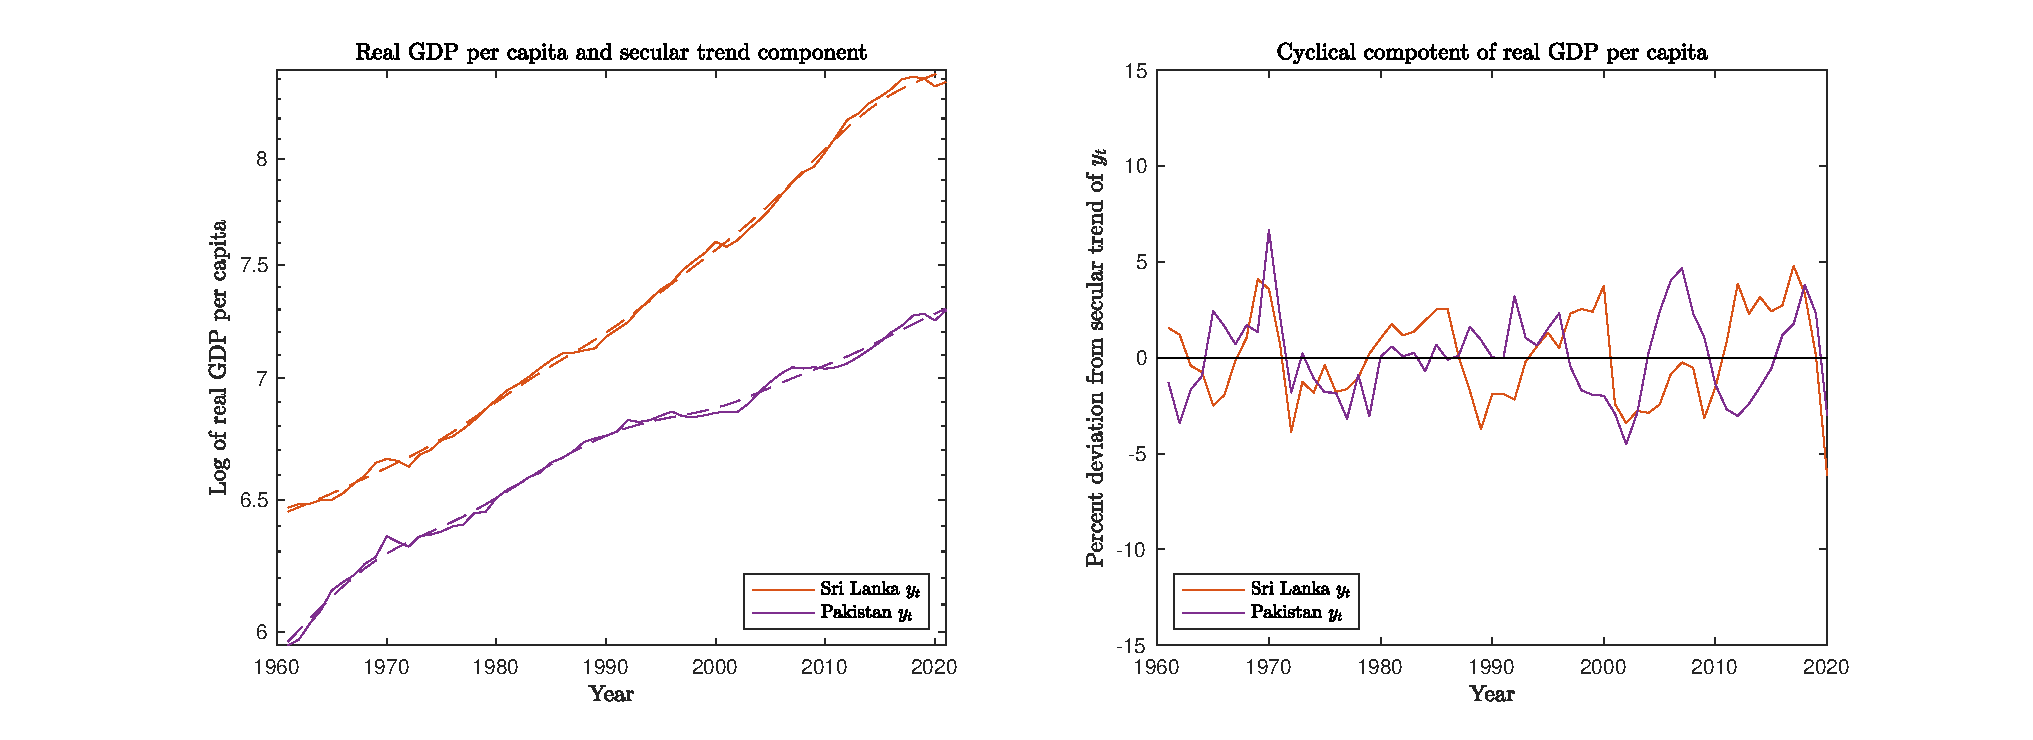
\includegraphics[width = \textwidth]{fig/decompose_gdp.eps}
    \caption{Decomposition of log-real-tradable-GDP for Sri Lanka and Pakistan}
    \label{fig:decompose-gdp}
    \floatfoot{\emph{Source:} World Bank national accounts data. \\
    \emph{Note:} The cyclical component in the right is obtained by the HP-filter with smoothing parameter $\lambda = 100$ for the log-real-GDP in the left. The quarterized AR(1) estimation for Sri Lanka yields $(\rho, \sigma_u)= (0.9114, 0.0123)$, and for Pakistan yields $(\rho, \sigma_u)= (0.9008, 0.0111)$}
\end{figure}
% \section*{}
\begin{landscape}
    % Please add the following required packages to your document preamble:
% \usepackage{booktabs}
% \usepackage{graphicx}
\begin{table}[h]
    \centering
    % \footnotesize
    \begin{tabular}{@{}lllH@{}}
    % \begin{tabular}{@{}lp{0.6\textwidth}lp{0.3\textwidth}@{}}
        \toprule
    Parameter  & Description                                                       & Value  & Source                                                                         \\ \midrule
    $\rho$     & Autocorrelation of output                                         & 0.9114  & Estimation of AR(1)\\
    $\sigma_u$ & Standard deviation of output                                      & 0.0123 & Estimation of AR(1) \\
    $r^*$      & Risk-free rate                                                    & 0.01 & 3 month treasury bill rate \\
    $\theta$   & Probability of reentry                                            & 0.0385 & \citet*{Reinhart-Rogoff-2014-100-episode}                                              \\
    $\alpha$   & Labor share in non-tradable goods sector                          & 0.65   & \citet{Jegajeevan-Sri-Lanka-DSGE}                                                       \\
    $a$        & Share of tradable consumption                                     & 0.35   &\citet*{Jegajeevan-Sri-Lanka-DSGE}                    \\
    $\xi$      & Intratemporal elasticity of substitution of consumption & 0.78   & \citet*{Jegajeevan-Sri-Lanka-DSGE}                              \\
    $\sigma$   & Inverse of intertemperal elasticity of substitution of consumption  & 1.28   & $1 / \xi$                                                                      \\
    $\beta$    & Discount factor                                                   & (\dots)  &                                                                                \\
    $\delta_1$ & Coefficient of the linear term in loss function                   &  (\dots) &                                                                                \\
    $\delta_2$ & Coefficient of the quadratic term in loss function                &  (\dots)   &                                                                                \\
    $\bar{h}$  & Labor endowment                                                   & 1      & Normalized to 1\\
    \bottomrule
    \end{tabular}%
    \caption{Calibration for Sri Lanka}
    \label{tab:cal-sri-lanka}
    \floatfoot{\emph{Note}: The time unit is one quarter. AR(1) is performed on annual tradable GDP data but quarterized following the approach of \citet*{Hinrichsen_2020-chapter4}. }
    \end{table}
    % Please add the following required packages to your document preamble:
% \usepackage{booktabs}
% \usepackage{graphicx}
\begin{table}[h]
    \centering
    % \footnotesize
    \begin{tabular}{@{}llll@{}}
    % \begin{tabular}{@{}lp{0.6\textwidth}lp{0.3\textwidth}@{}}
        \toprule
    Parameter  & Description                                                       & Value  & Source                                                                         \\ \midrule
    $\rho$     & Autocorrelation of output                                         & 0.9008  & Estimation of AR(1) on GDP\\
    $\sigma_u$ & Standard deviation of output                                      & 0.0111 & Estimation of AR(1) on GDP\\
    $r^*$      & Risk-free rate                                                    & 0.01 & 3 month treasury bill rate \\
    $\theta$   & Probability of reentry                                            & 0.0417 & \citet*{trebesch-2011-sovereign}                                              \\
    $\alpha$   & Labor share in non-tradable goods sector                          & 0.4   & \citet{Pakistan-DSGE-calibration}                                                       \\
    $a$        & Share of tradable consumption                                     & 0.33   &Share of tradable goods in GDP                    \\
    $\xi$      & Intratemporal elasticity of substitution of consumption & 0.5   & \citet{Na-18}                              \\
    $\sigma$   & Inverse of intertemperal elasticity of substitution of consumption  & 2   & $1 / \xi$                                                                      \\
    $\gamma$   & Downward wage rigidity                                            & 1.048   & \citet*{wage-rigidity-data}                  \\
    $\beta$    & Discount factor                                                   & (\dots)  &  Self-estimated \\
    $\delta_1$ & Coefficient of the linear term in loss function                   &  (\dots) &   Self-estimated  \\
    $\delta_2$ & Coefficient of the quadratic term in loss function                &  (\dots)   &     Self-estimated   \\
    $\bar{h}$  & Labor endowment                                                   & 1      & Normalized to 1\\
    \bottomrule
    \end{tabular}%
    \caption{Calibration for Pakistan}
    \label{tab:cal-pakistan}
    \floatfoot{\emph{Note}: The time unit is one quarter. AR(1) is performed on annual tradable GDP data but quarterized following the approach of \citet*{Hinrichsen_2020-chapter4}. }
    \end{table}
\end{landscape}


\begin{figure}[t]
    \centering
    \begin{subfigure}[t]{0.8\textwidth}
        \centering
        \includegraphics[width = \textwidth]{fig/default_set_sri_trad_hp.eps}
        \caption{Sri Lanka}
        \label{fig: ds-sri}
    \end{subfigure}%

    \begin{subfigure}[t]{0.8\textwidth}
        \centering
        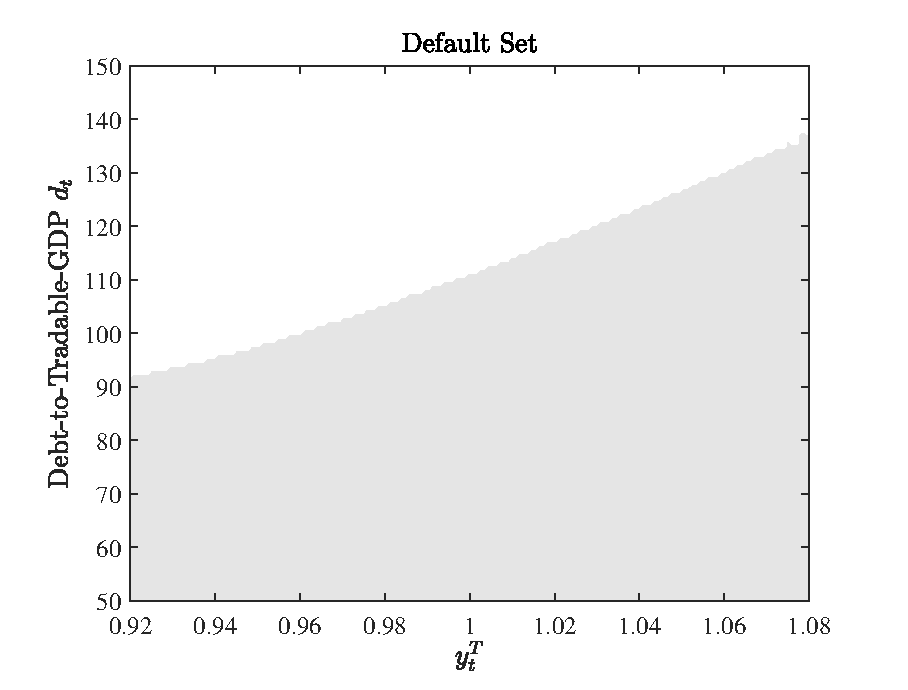
\includegraphics[width = \textwidth]{fig/default_set_pak_trad_hp.eps}
        \caption{Pakistan}
        \label{fig: ds-pak}
    \end{subfigure}
    \caption{Graphical Representation of Default Set}
    \label{fig:ds}
    \floatfoot{\emph{Note:} The default set derived via value function iteration is plotted on the state space. The horizontal axis represents the tradable output level, and the vertical axis represents the debt stock. The gray area represents the grid point where the country chooses not to default, and the white area is the grid point where default is the optimal action for the country.}
\end{figure}

\begin{figure}
    \begin{subfigure}[t]{0.8\textwidth}
        \includegraphics[width = \textwidth]{fig/default_set_sri_trad_hp_with_china.eps}
        \caption{Debt to All Creditors}
        \label{fig: ds-sri-data-with-china}
    \end{subfigure}

    \begin{subfigure}[t]{0.8\textwidth}
        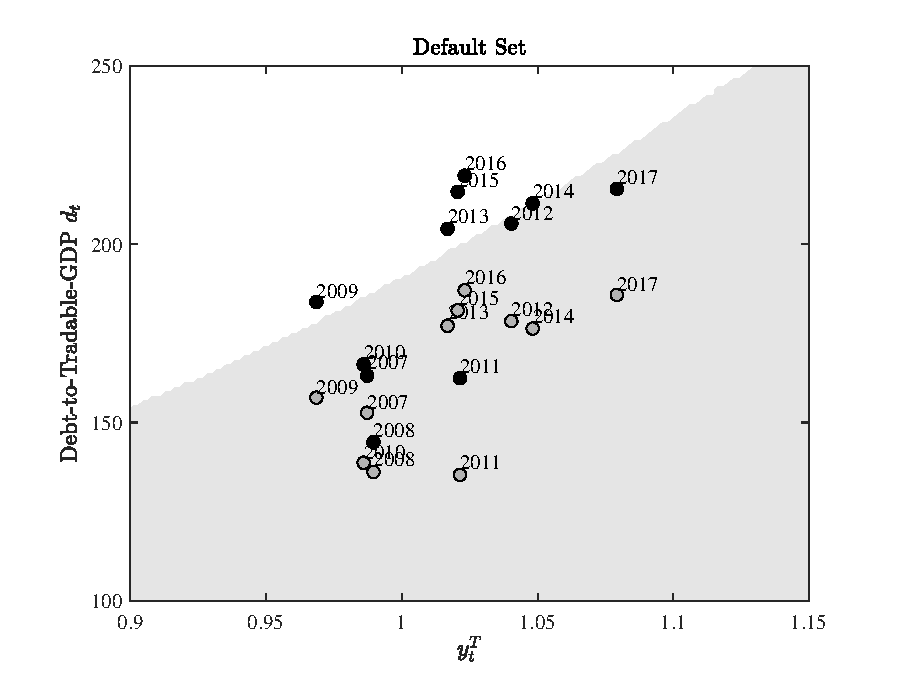
\includegraphics[width = \textwidth]{fig/default_set_sri_trad_hp_x_china.eps}
        \caption{Excluding Debt to China}
        \label{fig: ds-sri-data-x-china}
    \end{subfigure}
    \caption{Mapping Actual Data onto Analytical Model for Sri Lanka, 2007 -- 2017}
    \label{fig:ds-sri-data}
    \floatfoot{
        \emph{Source:} Debt data from IDS Database and \citet*{Horn-Reinhart-Trebesch-21} Database. GDP data from World Bank\\
        \emph{Note:} The gray region represents the non-default set of Sri Lanka, and the white region represents the default set. Black dots in (a) and (b) represents for the output-debt pair in the real data, and the gray dots in (b) represents the output-debt pair that excludes the debts from China.
    }
\end{figure}


\begin{figure}
    \begin{subfigure}[t]{0.8\textwidth}
        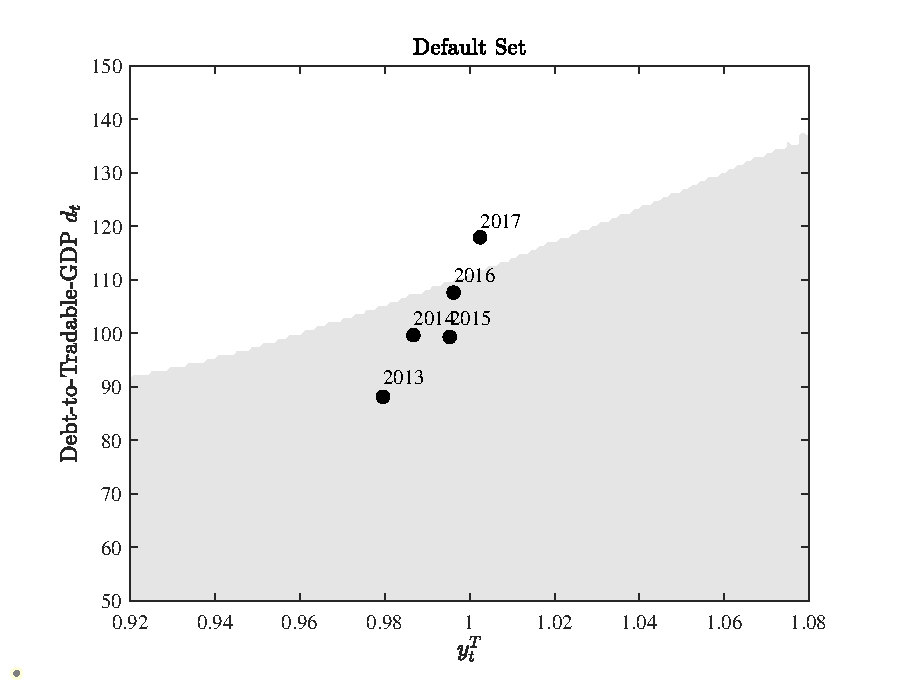
\includegraphics[width = \textwidth]{fig/default_set_pak_trad_hp_with_china.eps}
        \caption{Debt to All Creditors}
        \label{fig: ds-pak-data-with-china}
    \end{subfigure}

    \begin{subfigure}[t]{0.8\textwidth}
        \includegraphics[width = \textwidth]{fig/default_set_pak_trad_hp_x_china.eps}
        \caption{Excluding Debt to China}
        \label{fig: ds-pak-data-x-china}
    \end{subfigure}
    \caption{Mapping Actual Data onto Analytical Model for Pakistan, 2013 -- 2017}
    \label{fig:ds-pak-data}
    \floatfoot{
        \emph{Source:} Debt data from IDS Database and \citet*{Horn-Reinhart-Trebesch-21} Database. GDP data from World Bank\\
        \emph{Note:} The gray region represents the non-default set of Pakistan, and the white region represents the default set. Black dots in (a) and (b) represents for the output-debt pair in the real data, and the gray dots in (b) represents the output-debt pair that excludes the debts from China.
    }
\end{figure}


% \backmatter
\phantomsection
\addcontentsline{toc}{chapter}{\bibname}
\bibliographystyle{econ}

% Your bibliography goes here
\bibliography{bib/ref.bib}

\titleformat{\chapter}                      % 設置 Chapter 格式
{\Huge\bfseries}                            % 定義 format
{Appendix~\thechapter:~}              		        % 定義 label
{1em}                                       % 定義 sep
{}

\appendix
  \chapter{Output Loss}
  \label{ap: zarazaga}
  The following demonstrates the calculation of output loss associated with the default using the growth accounting approach proposed by \citet{zarazaga-12}.

Following \citet{zarazaga-12}, assume that the production function follows the form $y_t = h^\alpha_t k^{1-\alpha}_t$ where $y_t$ denotes output, $k_t$ denotes physical capital, and $h_t$ denotes employment.
This implies that by the relationship $\frac{y_t}{h_t} = \left( \frac{k_t}{y_t} \right)^{\frac{1-\alpha}{\alpha}}$. If the capital-output ratio before the default episode $\kappa_b =\frac{k_b}{y_b}$ falls to $\kappa_a = \frac{k_{a}}{y_a}$ after the default episode, the output per worker would be
$\Delta = \left[\left(\frac{\kappa_a}{\kappa_b} \right)^{\frac{1-\alpha}{\alpha}} -1\right]\times 100$ percent higher.
If we ascribe all the observed decrease to the sovereign default, we conclude that the output loss is on average $\frac{\Delta}{2} \%$ per worker during the period.
Note that $\left(\frac{\kappa_a}{\kappa_b} \right)^{\frac{1-\alpha}{\alpha}} -1 > 0$ if and only if $\kappa_a > \kappa_b$. This implies that there is an output loss only if the capital-output-ratio decreases. As argued in \citet{zarazaga-12}, the output loss is associated with a trough in the capital-output-ratio.

Using data from the Penn World Table, the annually capital-output ratio is calculated by dividing the capital stock at current PPPs (variable \emph{cn}) by the output-side real GDP at current PPPs (variable \emph{cgdpo}), both in million 2017 U.S. dollar.

In the case of Sri Lanka, capital-output ratio associated with the three default episodes (2005, 2012, 2017) recorded in the BoC-BoE Sovereign Default Database all increase, even for the consecutive years, as shown in Figure \ref{fig: sri-lanka-ky}. It is therefore unreasonable to attribute all the variations of the output to the sovereign default episodes.

For the case of Pakistan's biggest default in 1999, according to previous calibration, $\alpha=$ 0.4, which implies that by the relationship $\frac{y_t}{h_t} = \left( \frac{k_t}{y_t} \right)^{\frac{3}{2}}$.
The capital-output-ratio did not immediately fall after the crisis, but instead reached to 1.43 in 2003. It fell to about 1.347 in 2005, and slowly reached 1.6 in 2009, as shown in Figure \ref{fig: pakistan-ky}.
If $\frac{k_t}{y_t}$ had not fallen from 1.43 to 1.347 between 2003 to 2005, the output per worker would have been $ \left[\left(\frac{1.43}{1.347} \right)^{\frac{3}{2}} -1\right]\times 100$, approximately 9.84\% higher. Thus on average, the output per worker turned out to be $4.9\%$ lower if we ascribe all the fall in capital-to-output ratio to the default in 1999. Hence, we conclude that the output cost of the default for Pakistan in 1999 is 5\% per year per worker.


\begin{figure}[t]
    \centering
    \begin{subfigure}[position]{0.49\textwidth}
        \centering
        \includegraphics[width=\textwidth]{fig/sri_lanka_output_loss.pdf}
        \caption{Sri Lanka}
        \label{fig: sri-lanka-ky}
    \end{subfigure}
    \begin{subfigure}[position]{0.49\textwidth}
        \centering
        \includegraphics[width = \textwidth]{fig/pakistan_output_loss.pdf}
        \caption{Pakistan}
        \label{fig: pakistan-ky}
    \end{subfigure}
    \caption{Capital-Output Ratio, 1990 to 2020}
    \label{fig: LAK-PAK-ky}
    \floatfoot{Source: Penn World Table\\
    Note: The solid line represents the capital-output ratio for Sri Lanka and Pakistan. Default episode examined is plotted in vertical dashed lines.}
\end{figure}

  \chapter{Properties of the Default Set}
  \label{ap: default-set}
  In Chapter \ref{ch:model}, I introduce the default set given by the decentralized Eaton-Gersovitz model by \citet{Na-18}.
It is worth examining some properties of the default set, as it justifies visually the empirical results of the thesis.
Despite the fact that the default set can only be established through numerical computation instead of an analytical expression, some properties of the default set can still be obtained without knowing the exact form of the set.

\newcommand{\yT}{y^T_{t}}
\newcommand{\yTpr}{y^T_{t+1}}
\newcommand{\dpr}{d_{t+1}}
Recall that the default set is defined as
\begin{equation*}
    D(d_t) = \{\yT : v^b(\yT) > v^c(\yT, d_t)\},
\end{equation*}
which is the set of output levels within which the country is best to default given a debt level $d_t$.
I derive the following three properties regarding the default set under the model specifications of \citet{Na-18}:
\begin{enumerate}
    \item If the default set is not empty, then the trade balance deficit  is less that the loss. That is, $q(\yT, \dpr)\dpr - d_t < -L(\yT)$.
    \item If $y_1 \in D(d_t)$ and $\underline{y}\le y_2 \le y_1$, then $y_2 \in D(d_t)$
    \item The default set $D(d_t)$ is an interval $[\underline{y}, y^*(d_t)]$, where $y^*(d_t)$ is decreasing in $d_t$.
\end{enumerate}
Here, $\underline{y}$ denotes the lower bound on the endowment level during numerical computaiton.
Similar properties are proved in \citet*{Arellano-08} and \citet*{Uribe-Schmitt-Grohe-textbook} for the centralized version of Eaton-Gersovitz model.

\begin{proposition}
    \label{prop1}
    If $D(d_t) \neq \emptyset$, then $q(\yT, \dpr)\dpr - d_t < -L(\yT)$ for all $\dpr$.
\end{proposition}
\begin{proof}
    The proof is by contradiction. Suppose that $q(\yT, \tilde{d}_{t+1})\tilde{d}_{t+1} - d_t > -L(\yT)$ for some $\tilde{d}_t$, according to the definition of $v^c(d_t, \yT)$,
    \begin{align*}
        v^c(d_t, \yT) &= \max_{\dpr} \left\{
            U\left( A(\yT + q_t(\yT, \dpr) \dpr - d_t, \bar{h}) \right) +
            \beta E_t v^g(\yTpr, \dpr)
         \right\}\\
         &\ge U\left( A(\yT + q_t(\yT, \tilde{d}_{t+1}) \tilde{d}_{t+1} - d, \bar{h}) \right) +
            \beta E_t v^g(\yTpr, \tilde{d}_{t+1}) \\
         &\ge U\left( A(\yT -L(\yT), \bar{h}) \right) +
            \beta E_t v^b(\yTpr) \\
        &\equiv v^b(\yT).
    \end{align*}
    For third line, the first term holds due to the fact that both the utility function and the aggregation function is strictly increasing and concave, and the second term holds due to the definition of  $v^g = \max\{v^b, v^c\}$.

    This result, however, yields a contradiction since if $v^c(d_t, \yT) \ge v^b(\yT)$ for all possible endowments of tradable output, then we have $D(d_t) = \emptyset$ by definition. Therefore, we conclude that if under the certain debt level, the default set is not empty, then we must have $q(\yT, \dpr)\dpr - d_t < -L(\yT)$ for all $\dpr$.
\end{proof}

\begin{proposition}
    \label{prop2}
    If $y_1 \in D(d_t)$ and $\underline{y}\le y_2 \le y_1$, then $y_2 \in D(d_t)$.
\end{proposition}
\begin{proof}
    Consider the difference between the value function under bad standings $v^b(\yT)$ and the value function of continuing to repay its debt  $v^c(\yT, d_t)$ as $\Delta(\yT) \equiv v^b(\yT) - v^c(\yT, d_t)$. By definition, any tradable output in the default set $y \in D(d)$ satisfies $\Delta(y) >0$.

    Consider the first derivative of the difference function $\Delta_{y} = \pdv{\Delta}{y^T_t} = v^b_{y}(y) - v^c_{y}(y, d)$.
    Recall that
    \begin{align*}
        v^c(y, d) &= \max_{\left\{d' \right\}} \quad
        \left\{
            U\left(
                A\left( y + q(y, d')d' - d, F(1)\right)
             \right)
             + \beta E_t
             v^g \left(
                y', d'
              \right)
         \right\}\\
        v^b(y) &=
            U\left(
                A\left( y - L(y), F(1)\right)
             \right)
             + \beta E_t \left[
                \theta v^g \left(
                    y', 0
                \right)
                + (1-\theta) v^b \left(
                    y'
                 \right)
            \right].
    \end{align*}
    The notation for tradable output $y^T_t$ is simplified as $y$ and $y^T_{t+1}$ as $y'$, and similarly $d_t$ is simplified as $d$ and $d_{t+1}$ as $d'$. Also, from previous discussion we know that the optimal working hours is $h^*_t = \bar{h}$ when the government chooses to devaluate during default as its optimal policy, which is normalized to unity for simplicity. Applying the envelope theorem on $v^c(y, d)$,
    \begin{align*}
        v^c_y \equiv \pdv{v^c}{y} &= \pdv{}{y} U\Big[ A\Big(y + q(y, d')d' - d, F(1)\Big)\Big]\\
        &=\Big(1 + q_y(y, d')d'\Big) A_1(c_c, F(1)) U'\Big(A(c_c, F(1))\Big),
    \end{align*}
    where $q_y(y, d') \equiv \pdv{q}{y}$, $c_c \equiv y + q(y, d')d' -d$. This is easily derived by the chain rule. As for $v^b(y)$,
    \begin{align*}
        v^b_y \equiv \pdv{v^b}{y} &=
        \Big[ 1 - L' (y)\Big] A_1 (c_b, F(1)) U' \Bigl(A(c_b, F(1))\Bigr),
    \end{align*}
    where $L' \equiv \pdv{L}{y}$ and $c_b \equiv y - L(y)$
    For the sake of simplicity, the second parameter for the aggregation function $A(\cdot, \cdot)$ and its derivative $A_1(\cdot,\cdot )$ will be simplified by showing only the first argument since the second argument is always $F(1)$.

    Accordingly, the difference function
    \begin{align}
        \Delta_y =& v^b_y(y) - v^c_y(y, d) \nonumber \\
        =& \Big[ 1 - L' (y)\Big] A_1 (c_b) U' \Bigl(A(c_b)\Bigr)-
            \Big(1 + q_y(y, d')d'\Big) A_1(c_c) U'\Big(A(c_c)\Big) \nonumber\\
        =& A_1 (c_b) U' \Bigl(A(c_b)\Bigr)-A_1 (c_c) U' \Bigl(A(c_c)\Bigr)  \nonumber \\
        & -L'(y) A_1(c_b)U'(A(c_b)) - q_y(y, d')d'A_1(c_c)U'(c_c). \label{eq:diff-value-function}
    \end{align}

    Note that $A(\cdot, \cdot)$ and $U(\cdot)$ are both concave and increasing by assumption. This implies that if $c_1<c_2$, then
    \begin{enumerate*}[label = (\roman*)]
        \item $A(c_1) < A(c_2)$,
        \item $A_1(c_1) > A_1(c_2)$, and
        \item $U'(c_1) > U'(c_2)$
    \end{enumerate*}
    Together, it implies that $U'(A(c_1)) > U'(A(c_2))$. Furthermore, since $\frac{A_1(c_1)}{A_1(c_2)} > 1$ and $\frac {U'(A(c_1))}{U'(A(c_2))} > 1$, we have
    \begin{equation}
        \label{eq:AUA-compare}
        \frac{A_1(c_1) U'(A(c_1))}{A_1(c_2) U'(A(c_2))} > 1 \implies
        {A_1(c_1) U'(A(c_1))} > {A_1(c_2) U'(A(c_2))}.
    \end{equation}
    The first two terms in \refeq{eq:diff-value-function} resembles this relationship. Since
    \begin{equation*}
        c_b \equiv y - L(y) > y+q(y, d')d' -d \equiv c_c
    \end{equation*}
    according to Proposition \ref{prop1}, by \refeq{eq:AUA-compare}
    \begin{equation*}
        A_1 (c_b) U' \Bigl(A(c_b)\Bigr) - A_1 (c_c) U' \Bigl(A(c_c)\Bigr) < 0.
    \end{equation*}
    The third term in \refeq{eq:diff-value-function} is negative since the loss function is assumed to be nonnegative and nondecreasing \citep{Na-18}, hence $L'(y) > 0$. The marginal price of debt offered by foreign lenders $q_y(y, d')$ is positive since a better condition of output today $y$ yields a higher output tomorrow $y'$ due to the AR(1) nature of output, which in turn decreases the probability of default tomorrow. As a result, the price of bond increases.
    Overall, we have
    \begin{equation*}
        \Delta_y (y, d) < 0
    \end{equation*}
    if the default set is not empty. That is, $v^b(y) - v^c(y, d)$ is a decreasing function of $y$.

    When default is an optimal policy under the tuple $(y_1, d)$, which means that $y_1 \in D(d)$, then by definition $v^b(y_1) > v^c(y_1, d)$. For any given $y_2 \le y_1$, since $v^b(y) - v^c(y, d)$ is decreasing in $y$, we also have $v^b(y_2) > v^c(y_2, d)$, hence $y_2 \in D(d)$.
\end{proof}

\begin{proposition}
 The default set $D(d_t)$ is an interval $[\underline{y}, y^{T*}(d_t)]$, where $y^{T*}(d_t)$ is decreasing in $d_t$.
\end{proposition}
\begin{proof}
    Previously, it is proven that $\Delta_y(\yT, d_t) = v^b_y(\yT) - v^c_y(y^T_t, d_t) < 0$ when $D(d_t) \ne \emptyset$. An ouput is in the default set if $v^b(y^T_t) - v^c(y^T_t, d_t) >0$. It is trivial that as the output goes to infinity, the country has no incentive to default hence $v^c(\infty, d_t) > v^b(\infty)$. By the intermediate value theorem, it is obvious that there exist some $y^{T*}$ such that $v^b(y^{T*}) - v^c(y^{T*}, d_t) = 0$, where $y^{T*} = y^{T*}(d_t)$ is a value that depends on the current debt level. This proves that the default set is an interval.

    Taking the total derivative of the upper limit, together with the equation $\Delta(y^{T*}) = 0$, we get
    \begin{equation*}
        \dv{y^{T*}(d_t)}{d_t} = - \frac{\pdv{\Delta}{d_t}}{\pdv{\Delta}{y^{T}}} = - \frac{-v^c_d(y^{T*}(d_t), d_t)}{v^b_y(y^{T*}) - v^c_y(y^{T*}, d_t)}.
    \end{equation*}
    We know that $v^b_y(y^{T*}) - v^c_y(y^{T*}, d_tj) < 0$. Applying the envelope theorem to $v^c(y^{T*}_t, d_t)$, we get
    \begin{equation*}
        \pdv{v^c}{d_t} = -A_1\Big[y^{T*}_t + q_t(y^{T*}_t, \dpr)\dpr - d_t\Big] U'\Big[A(y^{T*}_t + q_t(y^{T*}_t, \dpr)\dpr - d_t)\Big]<0.
    \end{equation*}
    Eventually,
    \begin{equation}
        \dv{y^{T*}(d_t)}{d_t} > 0.
    \end{equation}

    This result replies that as the debt level increases, the upper bound of the default set should be strictly increasing.
\end{proof}

These results match those of \citet{Arellano-08} and \citet{Uribe-Schmitt-Grohe-textbook}. As discussed by \citet{Na-18}, when optimal devaluation and taxation policies are implemented, the equilibrium allocation in the economy aligns with that of the centralized Eaton-Gersovitz model. Therefore, it is not surprising that the default set in the decentralized economy exhibits similar behavior to that observed in a traditional centralized economy.

\end{document}
